%!TeX encoding = UTF-8
%!BIB program = biber

\documentclass[12pt,a4paper,UTF8,twocolumn]{ctexart}

\usepackage[top=2.5cm,bottom=2.5cm,left=2cm,right=2cm,bindingoffset=0.5cm]{geometry}
\usepackage{fancyhdr}
\usepackage{titlesec}
\usepackage{graphicx}
\usepackage{enumitem}
\usepackage{indentfirst}
\usepackage{amsmath}
\usepackage{url}
\usepackage{environ}
\usepackage{caption}
\usepackage{booktabs}
\usepackage{array}
\usepackage[most]{tcolorbox}
\usepackage[hidelinks]{hyperref}
\usepackage[backend=biber, style=gb7714-2015]{biblatex}

\addbibresource{ref.bib}

% 内建的功能 %
\newcommand{\fontstxs}{\fontsize{15pt}{17pt} \selectfont \songti{}}
\newcommand{\fontstsh}{\fontsize{14pt}{16pt} \selectfont \songti{}}
\newcommand{\fonthtxe}{\fontsize{18pt}{20pt} \selectfont \heiti{}}

\newcommand{\makecover}{
  \thispagestyle{empty}
  \begin{center}
    \vspace*{1cm}
    \noindent

    %% 这里两个minipage的作用是让Logo与标题对齐

    \begin{minipage}[c]{2.17cm}
      
\includegraphics[width=\linewidth]{assets/MUC.jpg}
    \end{minipage}
    \hspace{0.5cm}
    \begin{minipage}[c]{0.8\textwidth}
      {\fontsize{18pt}{20pt}\selectfont \heiti{}
      中央民族大学大学生创新训练计划结题论文\\[0.3cm]}
      {\fontsize{12pt}{14pt}\fontfamily{phv} \selectfont \bfseries
      URTP Final Thesis of Minzu University of China}

      % 中文黑体小二，英文Arial小四加粗
    \end{minipage}

    %% 下方是正式的内容

    \vspace{4cm}
    \makedoctitle{}
    \vspace{0.5cm}
    \makedocsubtitle{}
    \vspace{6cm}

    \begin{tabular}{ll}
      {\fontstxs{} 计划编号：} & \underline{\fontstxs{} \makebox[6cm][c]{\varmucprojectid}}\\
      {\fontstxs{} 项目类型：} & \underline{\fontstxs{} \makebox[6cm][c]{\varmucprojecttype}}\\
      {\fontstxs{} 指导教师：} & \underline{\fontstxs{} \makebox[6cm][c]{\varmucprojectteacher}}\\
      {\fontstxs{} 项目成员：} & \underline{\fontstxs{} \makebox[6cm][c]{\varmucprojectmembers}}\\
      {\fontstxs{} 依托单位：} & \underline{\fontstxs{} \makebox[6cm][c]{\varmucprojectunit}}\\
    \end{tabular}

    \vspace{3cm}

    {\fontstsh{} \varmucprojectdate{}}
  \end{center}
  \clearpage
}
\newcommand{\setupHeader}{
    \renewcommand{\baselinestretch}{1.25}
    \setlength{\parindent}{2em}
    \titleformat{\section}{\bfseries\heiti}{\thesection}{1em}{}
    \titlespacing*{\section}{0pt}{12pt}{6pt}
    
    \pagestyle{fancy}
    \setlength{\headheight}{14.5pt} % 建议值=基础值+2pt缓冲
    \setlength{\headsep}{15pt}      % 页眉与正文间距
    \fancyhf{}
    \fancyhead[C]{\songti\zihao{5}中央民族大学《纳米材料制备实验》课程论文}
    \renewcommand{\headrulewidth}{1pt} % 页眉线粗细
    \fancyfoot[C]{\thepage}
}
\makeatletter
\def\mucdoctitle{}
\makeatother

\newcommand{\doctitle}[1]{%
  \def\mucdoctitle{#1}%  不需要 \makeatletter，因为没用到 @
}

\newcommand{\makedoctitle}{%
  \color{white}\songti\zihao{3}%
  \mucdoctitle
}

\makeatletter
\def\mucdocsubtitle{}
\makeatother

\newcommand{\docsubtitle}[1]{%
  \makeatletter
  \def\mucdocsubtitle
{#1}%
  \makeatother
}

\newcommand{\makedocsubtitle}{%
  \makeatletter
  {\fontsize{16pt}{18pt} \selectfont \heiti{}%
\ifx\mucdocsubtitle\empty\else ——\mucdocsubtitle\fi}
  \makeatother
}

\makeatletter
\def\varmucprojectid{}
\makeatother

\newcommand{\mucprojectid}[1]{%
  \makeatletter
  \def\varmucprojectid{#1}%
  \makeatother
}

\makeatletter
\def\varmucprojecttype{}
\makeatother

\newcommand{\mucprojecttype}[1]{%
  \makeatletter
  \def\varmucprojecttype{#1}%
  \makeatother
}

\makeatletter
\def\varmucprojectteacher{}
\makeatother

\newcommand{\mucprojectteacher}[1]{%
  \makeatletter
  \def\varmucprojectteacher{#1}%
  \makeatother
}

\makeatletter
\def\varmucauthor{}
\makeatother

\newcommand{\mucauthor}[1]{%
  \makeatletter
  \def\varmucauthor{#1}%
  \makeatother
}

\makeatletter
\def\varmucstudentid{}
\makeatother

\newcommand{\mucstudentid}[1]{%
  \makeatletter
  \def\varmucstudentid{#1}%
  \makeatother
}

\makeatletter
\def\varmucclass{}
\makeatother

\newcommand{\mucclass}[1]{%
  \makeatletter
  \def\varmucclass{#1}%
  \makeatother
}

\newcommand{\makeauthorinfo}{%
  {%
    \begin{center}
      \par\noindent
      \songti\fontsize{16pt}{20pt}\selectfont
      \varmucauthor{}，\varmucclass{}，\varmucstudentid{}%
    \end{center}
  }%
}
\makeatletter
\def\muckeywords{} % @符号变量需包裹
\def\mucenglishkeywords{} % @符号变量需包裹
\makeatother

\newcommand{\keywords}[1]{%
  \makeatletter
  \def\muckeywords{#1}%
  \makeatother
}

% 关键词生成
\newcommand{\makekeywords}{%
  \makeatletter
  \par\noindent
  {\songti\fontsize{10pt}{\baselineskip}\textbf{关键字：}}%
  {\songti\fontsize{10pt}{\baselineskip}\space \muckeywords}
  \makeatother
}

\newsavebox{\abstractbox}
\newenvironment{MUCAbstract}{%
  \begin{lrbox}{\abstractbox}
    \minipage{\linewidth}  % 保证盒子宽度正常
    \songti\fontsize{10pt}{12pt}\selectfont
}{%
    \endminipage
  \end{lrbox}
  \phantomsection
  \addcontentsline{toc}{section}{摘要}%
  \noindent
  \songti\fontsize{10pt}{12pt}\selectfont
  \textbf{摘要：}\usebox{\abstractbox}%
  \par
}

\setupHeader{}

\newcommand{\sanhao}{\fontsize{15.6pt}{\baselineskip}\selectfont} % 三号
\newcommand{\sihao}{\fontsize{14pt}{\baselineskip}\selectfont}    % 四号
\newcommand{\xiaosi}{\fontsize{12pt}{14.4pt}\selectfont}          % 小四
\newcommand{\wuhao}{\fontsize{10.5pt}{12.6pt}\selectfont}         % 五号

\titleformat{\subsection}{\bfseries\songti\xiaosi}{\thesubsection}{1em}{}
\titleformat{\subsubsection}{\songti\xiaosi}{\thesubsubsection}{1em}{}
\setlist[enumerate,1]{label=(\arabic*),leftmargin=2em}
\setlist[enumerate,2]{label=\alph*.,leftmargin=4em}

\doctitle{热处理温度对溶胶-凝胶与静电纺丝 TiO$_2$ 纳米材料结构、形貌及光学性质的影响}
\keywords{二氧化钛；溶胶-凝胶法；静电纺丝；X 射线衍射；拉曼光谱；禁带宽度}
\mucauthor{刘佳鹏}
\mucstudentid{24012639}
\mucclass{24纳米2班}


\definecolor{titleGary}{rgb}{0.30, 0.44, 0.55}

\captionsetup{font=small,labelsep=quad}
\setlength{\columnsep}{0.9cm}
\renewcommand{\arraystretch}{1.15}
\xeCJKsetup{AutoFakeBold=2.5}
\renewcommand{\topfraction}{0.92}
\renewcommand{\bottomfraction}{0.7}
\renewcommand{\textfraction}{0.06}
\renewcommand{\floatpagefraction}{0.88}
\setcounter{topnumber}{4}
\setcounter{bottomnumber}{2}
\setcounter{totalnumber}{5}

\begin{document}

\twocolumn[{%
  \begin{flushright}
    
\includegraphics[width=2.8cm]{assets/MUC.jpg}
  \end{flushright}
  \vspace{-1.0cm}
  \begin{tcolorbox}[colback=titleGary, colframe=titleGary, sharp corners]
    \centering
    \color{white}\songti\zihao{4}\linespread{1.25}\selectfont
    \mucdoctitle{}
  \end{tcolorbox}
  \makeauthorinfo{}
  \makekeywords{}\par
  {\songti\fontsize{9.5pt}{13.5pt}\selectfont
\noindent\textbf{摘要：}以溶胶-凝胶法和静电纺丝法分别制备 TiO$_2$ 前驱体，并在空气气氛中经 200—900 $^\circ$C 保温 4 h 热处理，采用 X 射线衍射（XRD）、拉曼光谱、扫描电子显微镜与能谱（SEM/EDS）以及紫外-可见漫反射光谱对产物进行系统表征。结果表明：200 $^\circ$C 样品近于非晶态，仅呈现宽化的衍射包；300—600 $^\circ$C 产物为锐钛矿相，其 (101) 晶面衍射峰半高宽由 1.19$^\circ$ 收窄至 0.29$^\circ$，Scherrer 晶粒尺寸由 6.8 nm 增至 28.1 nm；700 $^\circ$C 起出现金红石相（质量分数 17.3\%），800 $^\circ$C 升至 84.7\%，900 $^\circ$C 完全转变为金红石。拉曼光谱中锐钛矿的 144、399、516、639 cm$^{-1}$ 特征峰随温度升高逐渐减弱，金红石的 448 和 611 cm$^{-1}$ 峰逐渐增强，与 XRD 结果一致；700 $^\circ$C 两个平行样品分别呈纯锐钛矿与纯金红石，说明相变在微区上并不均匀。SEM 统计得到 300、500、700 $^\circ$C 颗粒平均尺寸分别为 31$\pm$11、39$\pm$12、85$\pm$28 nm，900 $^\circ$C 时晶粒粗化至亚微米级；静电纺丝产物为直径中位数约 0.48 $\mu$m 的连续纤维，并伴有少量珠状缺陷。EDS 仅检出 Ti、O、C 及来自样品台的 Al，未发现其他杂质。由 Tauc 关系外推得到 400—600 $^\circ$C 样品的表观禁带宽度为 3.12—3.13 eV，700 $^\circ$C 降至 3.05 eV，800 $^\circ$C 进一步降至 2.80 eV。上述结果说明热处理温度通过“相变—晶粒生长—形貌粗化”的耦合过程同时调控 TiO$_2$ 的结构与光学性质，而制备路线主要影响产物的宏观组装形态。\par}

  \vspace{0.3em}
}]

\section{引\quad 言}

纳米材料的宏观性能并不只取决于化学组成，而在很大程度上由晶型、晶粒尺寸、形貌与表面状态共同决定；这些结构参数又可以在制备与后处理阶段被系统调控。在众多调控手段中，热处理最为简便：它既能提供相变所需的能量，又会驱动晶粒长大与颗粒烧结，因而是连接“制备”与“性能”的关键环节\cite{wang2005表征,li2008制备}。

二氧化钛是研究这一问题的理想模型体系。它存在锐钛矿、金红石和板钛矿三种晶型，其中锐钛矿为间接带隙半导体（约 3.2 eV），金红石为直接带隙半导体（约 3.0 eV）\cite{chen2007tio2}。热力学上金红石更稳定，但纳米尺度下表面能与晶粒尺寸会改变相稳定性，使相变温度随前驱体、杂质含量、气氛与升温制度在较宽区间内移动\cite{zhang2000phase}。同时，混相（锐钛矿/金红石）界面有利于电荷分离，往往比单一相具有更高的光催化活性\cite{ohtani1997mixture}，因此定量描述相变进程与晶粒长大规律具有实际意义。

从制备角度看，溶胶-凝胶法通过金属醇盐水解-缩聚获得均匀的前驱体，产物纯度高、组分易调，适合制备纳米颗粒；静电纺丝法则借助高压电场将溶胶拉伸成连续纤维，可获得高长径比、易回收的一维材料\cite{zhao2019静电纺丝}。两种路线得到的都是 TiO$_2$ 前驱体（水合氧化物/含聚合物复合纤维），后续热处理条件基本相同，这为比较“成型方式”与“热处理历史”对最终结构的影响提供了便利。

本文以第一轮专业实验中获得的 TiO$_2$ 系列样品为对象，选取溶胶-凝胶制备、静电纺丝制备、X 射线衍射、扫描电子显微镜与能谱、拉曼光谱、紫外-可见漫反射六个实验项目的数据开展分析。工作重点不在于复述各方法的原理，而是用同一温度序列（200—900 $^\circ$C）把四类表征结果串联起来，回答三个问题：(1) 相变发生在什么温度区间，转变程度如何随温度演化；(2) 晶粒与颗粒尺寸如何随温度长大，两者差异反映了什么结构特征；(3) 结构与形貌的变化如何体现在光学带隙上。通过交叉验证，期望给出一个可自洽解释的实验图像，并讨论其中的误差来源。

\section{实验原理与方法}

本文所用的实验项目、样品与测试条件汇总于表\ref{tab:projects}。两条制备路线均以钛酸四丁酯为前驱体，产物在相同温度序列下热处理，以保证后续比较的可比性。

\begin{figure*}[htbp]
  \centering
  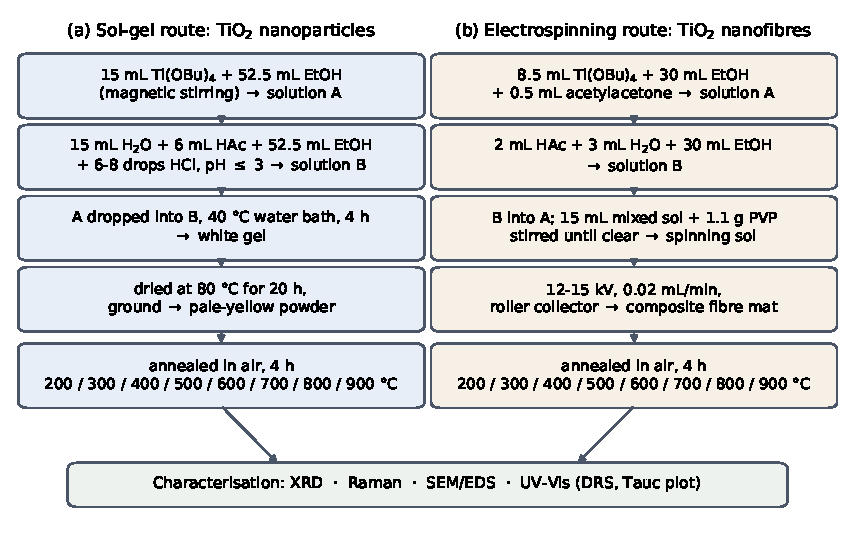
\includegraphics[width=0.86\textwidth]{figures/fig1_flow.pdf}
  \caption{溶胶-凝胶法 (a) 与静电纺丝法 (b) 的制备流程及后续表征示意}
  \label{fig:flow}
\end{figure*}

\begin{table}[htbp]
  \centering
  \caption{本文分析的实验项目与主要测试条件}
  \label{tab:projects}
  \footnotesize
  \begin{tabular}{@{}>{\raggedright\arraybackslash}p{2.05cm}>{\raggedright\arraybackslash}p{2.85cm}>{\raggedright\arraybackslash}p{1.9cm}@{}}
    \toprule
    实验项目 & 主要仪器/条件 & 数据来源 \\
    \midrule
    溶胶-凝胶制备 & 恒温水浴、马弗炉，200—900 $^\circ$C/4 h & 本文实验记录 \\
    静电纺丝制备 & PS-ZJ03 纺丝机，12—15 kV & 本文实验记录 \\
    X 射线衍射 & Cu $K\alpha$，20$^\circ$—80$^\circ$ & 第六组等 \\
    扫描电镜与能谱 & S-4800，10 kV，SE(U) & 第五组 \\
    拉曼光谱 & 633 nm 激发，50—1000 cm$^{-1}$ & 九组谱库 \\
    紫外-可见漫反射 & U-3900，300—600 nm & 第四组 \\
    \bottomrule
  \end{tabular}
\end{table}

\subsection{溶胶-凝胶法制备 TiO$_2$ 纳米颗粒}

溶胶-凝胶法的实质是金属醇盐的水解与缩聚：Ti(OBu)$_4$ 先与水反应生成羟基衍生物 Ti—OH，随后两个羟基（或羟基与残留烷氧基）缩合形成 Ti—O—Ti 桥键，逐渐构筑三维网络\cite{li2008制备}。体系中的冰醋酸既作为抑制剂与中心离子配位、降低水解速率，又通过调节 pH 使胶粒表面带同种电荷而避免团聚；盐酸将 pH 控制在 3 以下，进一步抑制过快水解，从而获得澄清、稳定的溶胶。溶胶在 40 $^\circ$C 水浴中经 4 h 交联老化形成白色凝胶，80 $^\circ$C 干燥 20 h 排出自由水与部分有机物，研磨后得到淡黄色干凝胶粉末，最后在空气气氛中于设定温度保温 4 h，完成有机残留的烧除与晶化。

具体配比与流程见图\ref{fig:flow}(a)：15 mL 钛酸四丁酯缓慢滴入 52.5 mL 无水乙醇得到溶液 A；15 mL 去离子水、6 mL 冰醋酸与 52.5 mL 无水乙醇混合后滴加 6—8 滴浓盐酸得到溶液 B；将 A 缓慢滴入 B 后于 40 $^\circ$C 反应 4 h。

\begin{table}[htbp]
  \centering
  \caption{溶胶-凝胶法制备 TiO$_2$ 的实验变量与预期结果}
  \label{tab:sg}
  \footnotesize
  \begin{tabular}{@{}p{2.4cm}p{4.1cm}@{}}
    \toprule
    实验变量 & 预期实验现象与结果 \\
    \midrule
    水量与酸量（pH） & 水量增大、pH 升高时水解加快，易生成沉淀；pH$\,\leq\,$3 时溶胶透明稳定 \\
    滴加顺序与速率 & A 滴入 B 且缓慢滴加时成胶均匀；滴加过快易局部水解产生颗粒团聚 \\
    水解温度 & 40 $^\circ$C 时缩聚速率适中；温度过高则凝胶时间缩短、孔径分布变宽 \\
    干燥条件 & 80 $^\circ$C 保温 20 h 可避免残存溶剂在煅烧时造成开裂 \\
    热处理温度 & 200—600 $^\circ$C 保持锐钛矿；700 $^\circ$C 起出现金红石；晶粒随温度长大 \\
    \bottomrule
  \end{tabular}
\end{table}

操作中需注意三点：其一，A 液滴入 B 液时必须缓慢并保持剧烈搅拌，防止局部浓度过高形成沉淀；其二，体系对水敏感，所用玻璃器皿需充分干燥；其三，干燥不充分的凝胶在高温煅烧时因溶剂急剧汽化而开裂，会破坏颗粒的均匀性。

\subsection{静电纺丝法制备 TiO$_2$ 纳米纤维}

静电纺丝利用高压静电场对聚合物溶液的作用实现纤维成型：液滴在针头处带电后同时受到外电场库仑力与表面电荷间的静电斥力，被拉伸成锥形（泰勒锥）；当电场强度超过临界值时，射流从锥顶喷出，在飞行过程中经历拉伸、鞭动、溶剂挥发与固化，最终以无纺布形式沉积在收集极上\cite{zhao2019静电纺丝}。本文以 PVP（$M\approx1.3\times10^{6}$）作为增稠与纺丝模板组分，它赋予溶胶足够的粘弹性以保证射流连续，并在后续煅烧中被完全烧除，留下 TiO$_2$ 纤维。

前驱体溶胶的配制见图\ref{fig:flow}(b)：8.5 mL 钛酸四丁酯与 0.5 mL 乙酰丙酮依次加入 30 mL 无水乙醇得到 A；2 mL 冰乙酸、3 mL 去离子水与 30 mL 无水乙醇混合得到 B；B 缓滴入 A 后取 15 mL 混合液加入 1.1 g PVP，室温搅拌至完全溶解且无气泡。纺丝时推进速率设为 0.02 mL/min，电压 12—15 kV，以滚筒为收集极。

\begin{table}[htbp]
  \centering
  \caption{静电纺丝法制备 TiO$_2$ 纤维的实验变量与预期结果}
  \label{tab:es}
  \footnotesize
  \begin{tabular}{@{}p{2.4cm}p{4.1cm}@{}}
    \toprule
    实验变量 & 预期实验现象与结果 \\
    \midrule
    PVP 含量 & PVP 过少时粘度过低、易形成液滴或珠粒；过多则纤维直径增大甚至堵塞针头 \\
    纺丝电压 & 低于临界电压时无法克服表面张力，无射流；过高则射流不稳定、纤维直径离散度增大 \\
    推进速率 & 速率过快使溶剂来不及挥发，纤维粘连并出现珠状缺陷 \\
    接收距离 & 距离过近易放电、溶剂残留；过远则电场强度下降、纤维变粗 \\
    环境湿度 & 湿度高时水分凝结，纤维表面出现孔洞或粘连 \\
    \bottomrule
  \end{tabular}
\end{table}

\subsection{表征方法与数据处理}

\textbf{X 射线衍射。} 衍射满足 Bragg 方程 $2d\sin\theta=n\lambda$，不同晶相具有唯一的衍射花样，据此可与标准 PDF 卡片比对完成物相鉴定\cite{shi2014xrd,zhou1999衍射}。测试采用 Cu $K\alpha$ 辐射（$\lambda=1.54056$ \AA），管压 40 kV、管流 30 mA，扫描范围 20$^\circ$—80$^\circ$，步宽 0.02$^\circ$。衍射数据以文本格式导出（含起始角、步宽、波长等文件头），分析时先用线性背景扣除，再用 pseudo-Voigt 函数对锐钛矿 (101)（$2\theta\approx25.3^\circ$）与金红石 (110)（$2\theta\approx27.4^\circ$）峰进行最小二乘拟合，得到峰位、半高宽与积分强度。晶粒尺寸由 Scherrer 公式估算：
\begin{equation}
  D=\frac{K\lambda}{\beta\cos\theta},
  \label{eq:scherrer}
\end{equation}
式中 $K=0.9$，$\beta$ 为半高宽（弧度），$\theta$ 为 Bragg 角。金红石的质量分数按直接对比法计算：
\begin{equation}
  X_{\mathrm{R}}=\frac{1}{1+0.8\,I_{\mathrm{A}}/I_{\mathrm{R}}},
  \label{eq:rutile}
\end{equation}
其中 $I_{\mathrm{A}}$、$I_{\mathrm{R}}$ 分别为锐钛矿 (101) 与金红石 (110) 的积分强度。

\textbf{拉曼光谱。} 拉曼散射反映分子与晶格的振动模式，对短程有序结构敏感，是 XRD 的重要补充\cite{wang2005表征}。测试采用 633 nm 激发，采集 50—1000 cm$^{-1}$ 区间。原始谱线先以非对称最小二乘（asLS）方法扣除荧光与瑞利背景，再用 Savitzky-Golay 滤波平滑，最后以 144 cm$^{-1}$ 峰（锐钛矿 $E_g$）归一化，以便比较不同温度样品的相对强度。

\textbf{扫描电镜与能谱。} SEM 通过聚焦电子束在样品表面逐点扫描、收集二次电子成像，可直接观察颗粒形貌与尺寸；EDS 则收集特征 X 射线给出元素组成\cite{huang2003分析}。测试在 Hitachi S-4800 上进行，加速电压 10 kV，工作距离 8.2—8.5 mm，信号为 SE(U)。粒径统计采用半自动方法：先由仪器导出的元数据读取像素标定（PixelSize，nm/像素），再对图像作高斯平滑、Otsu 阈值分割、距离变换与分水岭分离，最后按等效圆直径统计颗粒尺寸；对纤维样品则用骨架化后的距离变换值估计直径。该方法对粘连颗粒存在一定的主观性，故同时对分割结果作目视核查（见 3.3 节讨论）。

\textbf{紫外-可见漫反射。} 粉末样品在积分球中测得的吸光度 $A$ 与反射率 $R$ 满足 $A=-\lg R$。为消除散射差异，用 Kubelka-Munk 函数将其转换为吸收系数：
\begin{equation}\small
  F(R)=(1-R)^2/2R,
  \label{eq:km}
\end{equation}
再由 Tauc 关系外推表观带隙：
\begin{equation}\small
  [\,F(R)\,h\nu\,]^{1/2}=A\,(h\nu-E_g),
  \label{eq:tauc}
\end{equation}
锐钛矿为间接带隙半导体，故取指数 1/2。测试条件为 300—600 nm、扫描速率 600 nm/min、采样间隔 0.5 nm、狭缝 4 nm，以白板作基线。


\section{结果与讨论}

\subsection{物相组成与相变行为}

图\ref{fig:xrd}给出同一系列样品（第六组）在 200—900 $^\circ$C 热处理后的 XRD 图谱。200 $^\circ$C 样品在 25$^\circ$ 附近仅有一个宽化的包峰，半高宽达 1.19$^\circ$，其余位置没有可分辨的衍射峰，说明该温度下产物仍以非晶或极细的纳米晶形式存在，热处理尚未提供足够的晶化能。300 $^\circ$C 起图谱中出现明确的锐钛矿衍射峰，峰位与 PDF 卡片（锐钛矿 JCPDS 21-1272、金红石 JCPDS 21-1276）对应的 (101)、(004)、(200)、(105)、(211) 等晶面一致，峰形随温度升高而显著锐化，表明晶化程度与晶粒尺寸同步提高。

\begin{figure}[htbp]
  \centering
  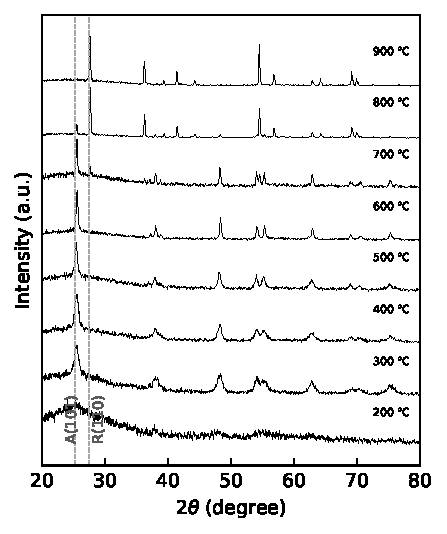
\includegraphics[width=\linewidth]{figures/fig2_xrd_stack.pdf}
  \caption{不同热处理温度下 TiO$_2$ 样品的 XRD 图谱（第六组，2$\theta$=20$^\circ$—80$^\circ$）。虚线分别标出锐钛矿 A(101) 与金红石 R(110) 的标准峰位}
  \label{fig:xrd}
\end{figure}

700 $^\circ$C 时在 27.4$^\circ$ 处出现金红石 (110) 衍射峰，同时 25.3$^\circ$ 的锐钛矿峰仍然存在，说明此时处于两相共存阶段；800 $^\circ$C 时金红石峰成为最强峰，锐钛矿峰明显减弱；900 $^\circ$C 时锐钛矿峰完全消失。各温度下观察到的主要峰位及其归属列于表\ref{tab:peaks}。

\begin{table}[htbp]
  \centering
  \caption{各温度样品主要衍射峰的归属（PDF 标准值对比）}
  \label{tab:peaks}
  \footnotesize
  \begin{tabular}{@{}cccc@{}}
    \toprule
    $2\theta_{\mathrm{obs}}/(^\circ)$ & $2\theta_{\mathrm{PDF}}/(^\circ)$ & $(hkl)$ & 物相 \\
    \midrule
    25.4—25.6 & 25.28 & (101) & 锐钛矿 \\
    37.8      & 37.80 & (004) & 锐钛矿 \\
    48.0      & 48.05 & (200) & 锐钛矿 \\
    54.0      & 53.89 & (105) & 锐钛矿 \\
    55.1      & 55.06 & (211) & 锐钛矿 \\
    27.5      & 27.45 & (110) & 金红石 \\
    36.2      & 36.09 & (101) & 金红石 \\
    41.2      & 41.23 & (111) & 金红石 \\
    54.3      & 54.32 & (211) & 金红石 \\
    56.6      & 56.64 & (220) & 金红石 \\
    \bottomrule
  \end{tabular}
\end{table}

值得指出的是，本文拟合得到的锐钛矿 (101) 峰位在 25.45$^\circ$—25.56$^\circ$ 之间，系统性地高于标准值 25.28$^\circ$ 约 0.2$^\circ$。这一偏差并未随温度单调变化，更可能源于样品表面与样品槽不共面引起的样品位移误差以及仪器零点漂移，而不是晶格畸变，因此在后续定量分析中仅使用同一温度序列内的相对变化。

图\ref{fig:xrdq}与表\ref{tab:xrdq}给出了峰宽、晶粒尺寸与金红石含量的定量结果。晶粒尺寸由 200 $^\circ$C 的 6.8 nm 单调增至 800 $^\circ$C 的 44.8 nm，增长曲线呈现明显的两段特征：300—500 $^\circ$C 区间增长缓慢（9.9→16.9 nm），500—800 $^\circ$C 区间增长加快（16.9→44.8 nm）。这种“先慢后快”的行为说明低温阶段晶粒长大受限于表面扩散与晶界迁移的动力学势垒，而温度超过约 500 $^\circ$C 后热激活使晶界迁移速率显著提高。金红石含量在 200—600 $^\circ$C 始终保持为零，700 $^\circ$C 突增至 17.3\%，800 $^\circ$C 达到 84.7\%，900 $^\circ$C 为 100\%，呈典型的 S 形转变特征，符合“成核—长大”型相变规律：只有当锐钛矿晶粒长大到某一临界尺寸、金红石晶核能够稳定存在时，相变才会迅速推进\cite{zhang2000phase}。

\begin{figure}[htbp]
  \centering
  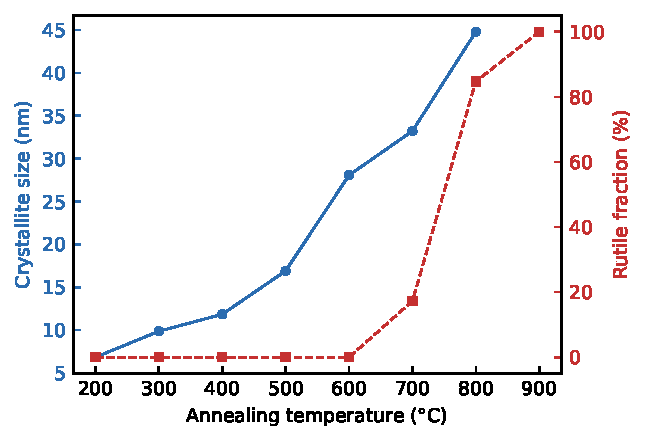
\includegraphics[width=\linewidth]{figures/fig3_xrd_quant.pdf}
  \caption{锐钛矿 (101) 峰对应的 Scherrer 晶粒尺寸与金红石质量分数随热处理温度的变化}
  \label{fig:xrdq}
\end{figure}

\begin{table}[htbp]
  \centering
  \caption{不同热处理温度下的半高宽、晶粒尺寸与金红石含量}
  \label{tab:xrdq}
  \footnotesize
  \begin{tabular}{@{}cccc@{}}
    \toprule
    $T/^\circ$C & FWHM$(101)/(^\circ)$ & $D$/nm & $X_{\mathrm{R}}$/\% \\
    \midrule
    200 & 1.19 & 6.8  & 0 \\
    300 & 0.83 & 9.9  & 0 \\
    400 & 0.69 & 11.8 & 0 \\
    500 & 0.48 & 16.9 & 0 \\
    600 & 0.29 & 28.1 & 0 \\
    700 & 0.25 & 33.2 & 17.3 \\
    800 & 0.18 & 44.8 & 84.7 \\
    900 & ---  & ---  & 100.0 \\
    \bottomrule
  \end{tabular}
\end{table}

为检验结果的可靠性，本文把四个小组在相同温度下的数据做了横向比较（图\ref{fig:groups}）。四组的晶粒尺寸随温度的变化趋势基本重合，在 700 $^\circ$C 均落在 33—41 nm 区间；金红石含量的变化也大体一致。个别数据点偏离趋势：某一小组 800 $^\circ$C 样品未检出金红石且晶粒尺寸偏小（18.4 nm），另一小组 200 $^\circ$C 样品的晶粒尺寸偏大（13.6 nm）。考虑到四组使用的是同一批前驱体与同一台仪器，这类偏离更可能来自装样高度不一致、样品量差异或粉末压实程度不同造成的峰形变化，而非真实的物相差异。这提示在定量比较时，应尽量保证样品制备与装样条件的一致性。

\begin{figure*}[htbp]
  \centering
  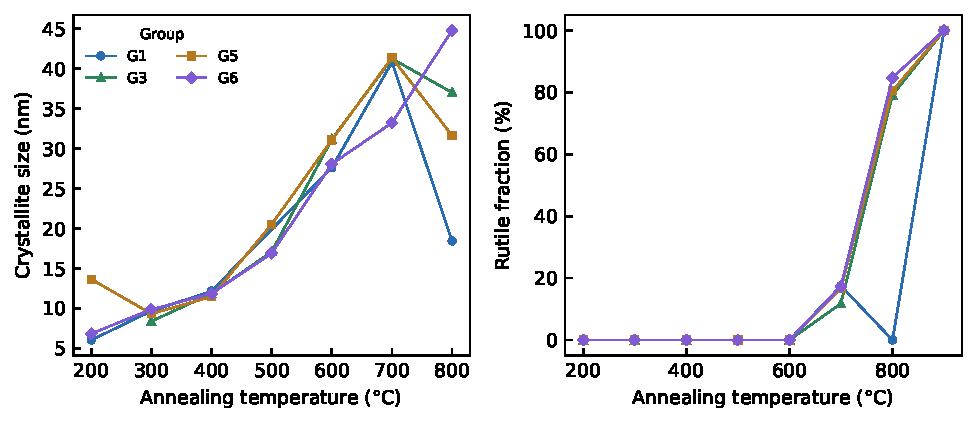
\includegraphics[width=0.74\textwidth]{figures/fig4_xrd_groups.pdf}
  \caption{四个小组数据的重复性比较：(a) 晶粒尺寸；(b) 金红石质量分数随温度的变化}
  \label{fig:groups}
\end{figure*}

\subsection{拉曼光谱对局域结构的验证}

XRD 给出的是长程平均结构信息，而拉曼光谱对短程有序与局域成键更敏感。图\ref{fig:raman}为不同温度样品的拉曼谱（已扣除荧光背景并按 144 cm$^{-1}$ 峰归一化）。400、500、600 $^\circ$C 样品在 144、396—399、515—517 和 639—642 cm$^{-1}$ 处出现清晰谱峰，与锐钛矿的 $E_g$、$B_{1g}$、$A_{1g}+B_{1g}$ 和 $E_g$ 振动模式一一对应；其中 144 cm$^{-1}$ 峰强度最大、随温度升高半高宽逐渐变窄，说明 TiO$_6$ 八面体骨架的短程有序度不断提高，与 XRD 中峰形锐化的结论互相印证。

\begin{figure*}[htbp]
  \centering
  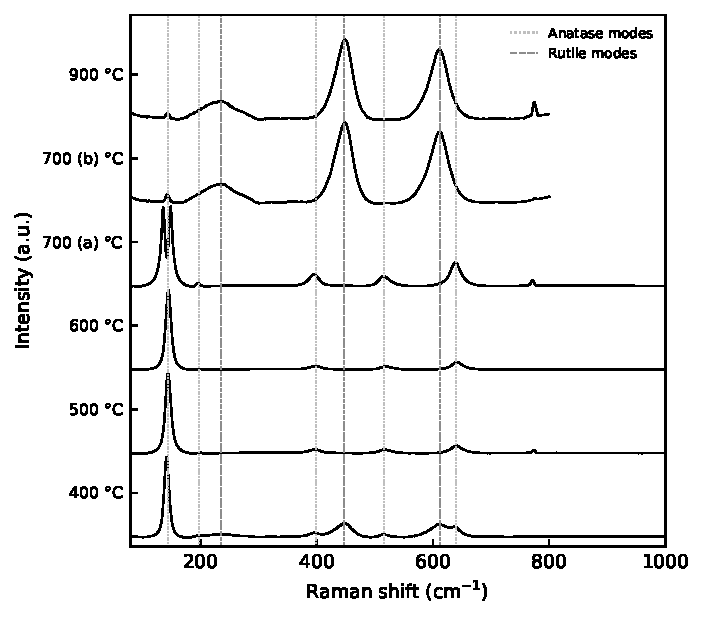
\includegraphics[width=0.56\textwidth]{figures/fig5_raman.pdf}
  \caption{不同热处理温度下 TiO$_2$ 的拉曼光谱（633 nm 激发，已作基线校正与归一化）。点线为锐钛矿特征模式位置，虚线为金红石特征模式位置；700 $^\circ$C 的两个平行样品分别记为 (a) 与 (b)}
  \label{fig:raman}
\end{figure*}

700 $^\circ$C 的两个平行样品呈现出截然不同的谱形：样品 (a) 仍以 149 cm$^{-1}$ 的锐钛矿峰为主，同时 395、515、639 cm$^{-1}$ 峰依然清晰；样品 (b) 则在 143、233、448 和 611 cm$^{-1}$ 处出现金红石的特征峰，其中 448 cm$^{-1}$（$E_g$）与 611 cm$^{-1}$（$A_{1g}$）强度最高。900 $^\circ$C 样品的谱形与样品 (b) 一致，锐钛矿峰完全消失。XRD 给出的 700 $^\circ$C 平均金红石含量为 17.3\%，而拉曼在微米级光斑内却分别观察到“纯锐钛矿”和“纯金红石”两种状态，说明相变在微区尺度上分布极不均匀——这可能与炉内温度梯度、样品堆积厚度导致的局部热历史差异有关。这也解释了为何不同小组在 700 $^\circ$C 附近给出的相含量数据分散度最大。

\begin{table}[htbp]
  \centering
  \caption{拉曼特征峰位及其振动模式归属}
  \label{tab:raman}
  \footnotesize
  \setlength{\tabcolsep}{3pt}
  \begin{tabular}{@{}lccc@{}}
    \toprule
    物相 & 文献/cm$^{-1}$ & 观测/cm$^{-1}$ & 振动模式 \\
    \midrule
    锐钛矿 & 144 & 142—149 & $E_g$ \\
           & 197 & 197     & $E_g$ \\
           & 399 & 395—399 & $B_{1g}$ \\
           & 516 & 515—517 & $A_{1g}+B_{1g}$ \\
           & 639 & 639—642 & $E_g$ \\
    金红石 & 233 & 233     & 多声子过程 \\
           & 447 & 448     & $E_g$ \\
           & 612 & 610—611 & $A_{1g}$ \\
    \bottomrule
  \end{tabular}
\end{table}

\subsection{形貌演化与粒径统计}

图\ref{fig:sem}给出五个温度点的 SEM 形貌像。200 $^\circ$C 样品表面致密平整，除少量碎屑外看不到可分辨的颗粒，这与 XRD 中宽化包峰所反映的非晶/极细晶状态一致；300 $^\circ$C 时表面出现密集的细小颗粒，边界模糊，平均尺寸约 31 nm；500 $^\circ$C 时颗粒轮廓清晰、尺寸分布较窄，平均 39 nm；700 $^\circ$C 时颗粒明显长大并出现棱角分明的多面体外形，平均 85 nm；900 $^\circ$C 时晶粒已粗化至亚微米尺度，部分区域出现明显的烧结颈与孔洞，说明此时颗粒间已发生显著的固相烧结。

\begin{figure*}[htbp]
  \centering
  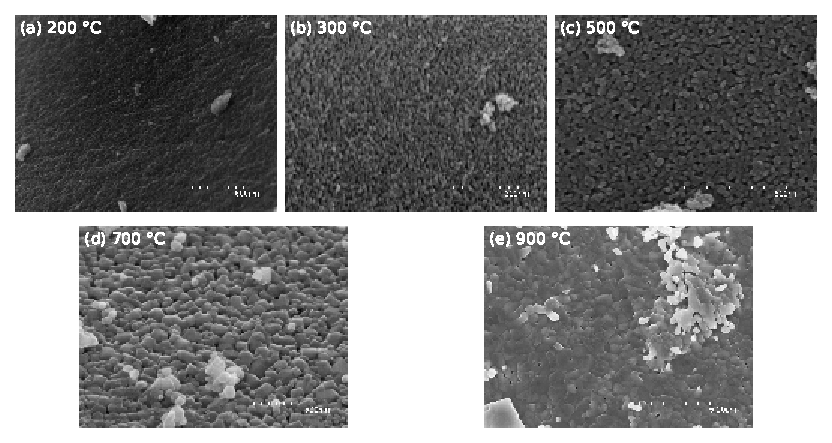
\includegraphics[width=0.74\textwidth]{figures/fig6_sem.pdf}
  \caption{不同热处理温度下 TiO$_2$ 样品的 SEM 形貌：(a) 200 $^\circ$C；(b) 300 $^\circ$C；(c) 500 $^\circ$C；(d) 700 $^\circ$C；(e) 900 $^\circ$C（图中标尺为仪器原始标尺）}
  \label{fig:sem}
\end{figure*}

图\ref{fig:hist}为 300、500、700 $^\circ$C 样品的粒径分布直方图，统计结果汇总于表\ref{tab:size}。三个温度下的分布均近似单峰且略有右偏，标准差随温度升高而增大（11→28 nm），说明高温下颗粒生长的随机性增强。将 SEM 统计的颗粒尺寸与 XRD 的晶粒尺寸比较可以发现，两者相差约 1.5—2.5 倍：500 $^\circ$C 时颗粒 39 nm 而晶粒 16.9 nm，700 $^\circ$C 时颗粒 85 nm 而晶粒 33.2 nm。这一差异说明 SEM 观察到的“颗粒”多为若干一次晶粒构成的聚集体，颗粒内部仍存在晶界；同时也提醒在用不同方法表征“尺寸”时必须明确所指的物理量。

\begin{figure*}[htbp]
  \centering
  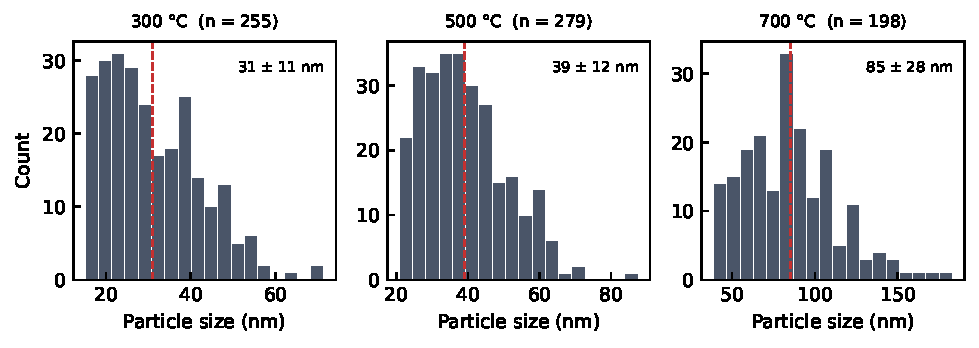
\includegraphics[width=0.72\textwidth]{figures/fig7_sem_hist.pdf}
  \caption{300、500、700 $^\circ$C 样品的粒径分布（虚线为平均值）}
  \label{fig:hist}
\end{figure*}

\begin{table}[htbp]
  \centering
  \caption{SEM 粒径统计结果}
  \label{tab:size}
  \footnotesize
  \setlength{\tabcolsep}{2.4pt}
  \begin{tabular}{@{}ccccc@{}}
    \toprule
    $T/^\circ$C & nm/px & $N$ & $d$/nm & 中位数/nm \\
    \midrule
    200 & 2.83 & --- & 无明显颗粒 & --- \\
    300 & 1.32 & 255 & 31$\pm$11 & 28 \\
    500 & 1.80 & 279 & 39$\pm$12 & 37 \\
    700 & 2.83 & 198 & 85$\pm$28 & 83 \\
    900 & 18.04 & 64 & 942$\pm$622 & 743 \\
    \bottomrule
  \end{tabular}
\end{table}

作为对照，静电纺丝产物的形貌与上述颗粒体系完全不同。纺丝得到的是一层连续的无纺纤维膜，纤维直径中位数约 0.48 $\mu$m（由骨架距离变换统计，$n\approx2.7\times10^{4}$ 个采样点，均值 0.61 $\mu$m、标准差 0.41 $\mu$m），纤维之间存在大量交叉搭接，从而形成高孔隙率的网络结构；同时可观察到直径数微米的珠状缺陷（beads），这是射流在飞行过程中表面张力占优、未能充分拉伸所致，与表\ref{tab:es}中关于浓度、电压与推进速率的分析一致。纤维形貌使该路线产物在比表面积与回收便利性上优于粉体，但在相同热处理条件下其相组成仍由温度决定。

\subsection{能谱分析}

图\ref{fig:eds}为 500 与 900 $^\circ$C 样品的 EDS 谱。两张谱中均只出现 C $K\alpha$（0.28 keV）、O $K\alpha$（0.53 keV）、Ti $L\alpha$（0.45 keV）、Ti $K\alpha$（4.51 keV）与 Ti $K\beta$（4.93 keV）等特征峰，未检出其他金属杂质；1.49 keV 处的弱峰对应 Al $K\alpha$，来自承载样品的铝基底或样品台。C 信号强度随温度升高而下降，与高温下有机残留被充分烧除、表面吸附碳减少的规律一致。需要说明的是，受样品表面粗糙度与计数率限制，本次测试只做了定性成分确认，未进行定量归一化，因此不宜据此讨论 Ti/O 原子比。

\begin{figure}[htbp]
  \centering
  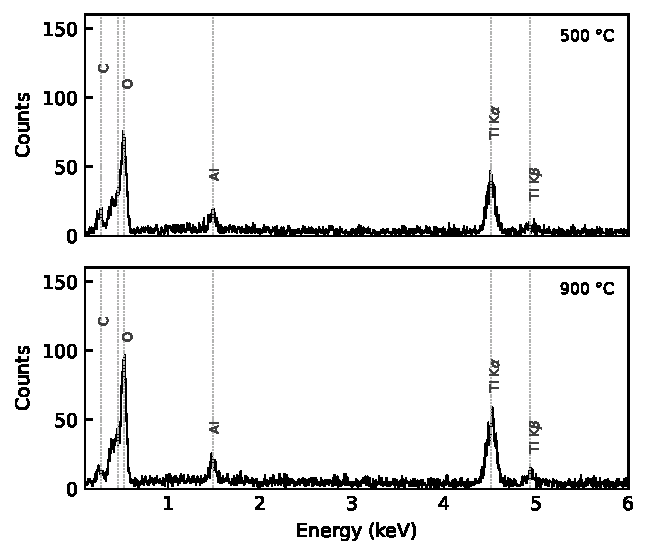
\includegraphics[width=\linewidth]{figures/fig8_eds.pdf}
  \caption{500 $^\circ$C 与 900 $^\circ$C 样品的 EDS 谱（10 kV）}
  \label{fig:eds}
\end{figure}

\subsection{光学性质与带隙}

图\ref{fig:uv}为 400—800 $^\circ$C 样品的紫外-可见吸收谱。所有样品在 400 nm 以下均表现出强吸收，吸收边随热处理温度升高逐渐向长波方向移动：400—600 $^\circ$C 样品的吸收边约在 390 nm，700 $^\circ$C 移至约 400 nm，800 $^\circ$C 进一步红移至约 415 nm。这一红移与金红石相的出现及晶粒长大相对应，因为金红石的带隙（约 3.0 eV）小于锐钛矿（约 3.2 eV），且晶粒增大使量子尺寸效应减弱\cite{serpone1995size}。

\begin{figure}[htbp]
  \centering
  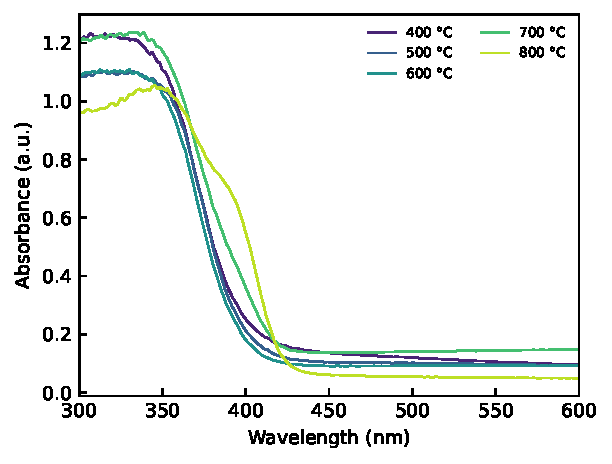
\includegraphics[width=\linewidth]{figures/fig9_uvvis.pdf}
  \caption{不同热处理温度下 TiO$_2$ 的紫外-可见吸收光谱}
  \label{fig:uv}
\end{figure}

将吸收谱按式\eqref{eq:km}与式\eqref{eq:tauc}转换为 Tauc 曲线（图\ref{fig:tauc}），对吸收边线性段作切线外推，得到各样品的表观带隙（表\ref{tab:eg}）：400、500、600 $^\circ$C 分别为 3.12、3.12、3.13 eV，与锐钛矿的文献值 3.2 eV 接近而略低，可能与纳米颗粒表面态及氧空位引起的带尾吸收有关；700 $^\circ$C 降至 3.05 eV，800 $^\circ$C 进一步降至 2.80 eV，与金红石含量由 17.3\% 增至 84.7\% 的趋势一致。800 $^\circ$C 样品的 Tauc 曲线在 3.0 eV 附近存在明显的肩部，线性区判定对 Eg 的影响可达 $\pm0.05$ eV，因此该数值应视为上限估计。

\begin{figure}[htbp]
  \centering
  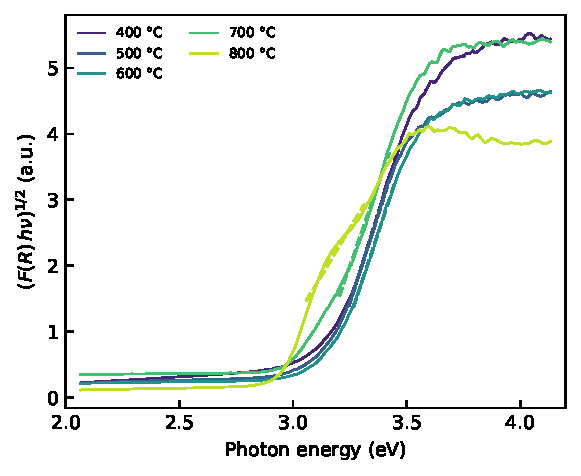
\includegraphics[width=\linewidth]{figures/fig10_tauc.pdf}
  \caption{由 Kubelka-Munk 函数转换得到的 Tauc 曲线及线性外推（虚线）}
  \label{fig:tauc}
\end{figure}

\begin{table}[htbp]
  \centering
  \caption{各温度样品的表观禁带宽度}
  \label{tab:eg}
  \footnotesize
  \begin{tabular}{@{}cccc@{}}
    \toprule
    $T/^\circ$C & 主要物相 & $X_{\mathrm{R}}$/\% & $E_g$/eV \\
    \midrule
    400 & 锐钛矿 & 0    & 3.12 \\
    500 & 锐钛矿 & 0    & 3.12 \\
    600 & 锐钛矿 & 0    & 3.13 \\
    700 & 锐钛矿+金红石 & 17.3 & 3.05 \\
    800 & 金红石为主 & 84.7 & 2.80 \\
    \bottomrule
  \end{tabular}
\end{table}

需要说明的是，900 $^\circ$C 样品的吸收谱基线未正确归零（吸光度出现负值），数据不可靠，故未纳入带隙分析。这一细节也提示在漫反射测试中，参比白板的清洁度与基线扫描步骤对结果影响很大。

\subsection{综合讨论}

把四类表征结果放在同一温度坐标下，可以得到一条自洽的演化链条：200 $^\circ$C 时前驱体尚未完成晶化，产物近于非晶；300—600 $^\circ$C 区间锐钛矿晶粒由 10 nm 长到 28 nm，颗粒由 31 nm 长到 39 nm，禁带宽度稳定在 3.12—3.13 eV；700 $^\circ$C 是相变的临界区间，金红石开始成核并快速长大，微区上锐钛矿与金红石并存，宏观带隙下降；800—900 $^\circ$C 金红石成为主相甚至唯一相，晶粒与颗粒同时粗化至亚微米级，带隙进一步红移。相变温度（600—700 $^\circ$C）与溶胶-凝胶法 TiO$_2$ 的文献报道一致\cite{zhang2000phase,chen2007tio2}，说明本文的热处理制度是合理的。

制备路线的作用主要体现在宏观组装形态上：溶胶-凝胶法得到的是颗粒堆积体，颗粒之间以点接触为主，比表面积大但回收困难；静电纺丝法得到的是连续纤维膜，纤维直径约 0.5 $\mu$m，长径比高、易于分离回收，但存在珠状缺陷。两者在相同温度下的相变行为并无本质差异，说明决定相组成的仍是热处理历史而非成型方式。若面向光催化应用，可考虑利用纤维膜的可回收性，并通过控制煅烧温度在锐钛矿/金红石混合相区间（约 700 $^\circ$C）获得有利于电荷分离的界面结构\cite{ohtani1997mixture}。

本文的分析仍存在若干不足。其一，Scherrer 公式未扣除仪器宽化与晶格应变，所得晶粒尺寸为表观下限值，对于 200 $^\circ$C 这类峰形严重宽化的样品误差更大；其二，金红石含量采用直接对比法，只使用了一对衍射峰，未做 Rietveld 全谱精修，绝对误差估计为 $\pm5\%$；其三，SEM 粒径统计依赖半自动分割，对粘连颗粒存在过分割或漏分割，人工核查估计相对误差约 10\%—15\%；其四，漫反射谱只测量了 300—600 nm，未覆盖近红外区，Tauc 外推的线性区选择带有主观性。后续若能补充 Rietveld 精修、BET 比表面积与 TEM 观察，将能更准确地描述“晶粒—颗粒—团聚体”的多级结构。





\section{结\quad 论}

本文以溶胶-凝胶与静电纺丝两条路线制备的 TiO$_2$ 为对象，用 XRD、拉曼光谱、SEM/EDS 与紫外-可见漫反射对同一温度序列（200—900 $^\circ$C）的产物进行了系统表征，主要结论如下。

(1) 相变过程具有明确的温度阈值与 S 形特征。200 $^\circ$C 样品近于非晶；300—600 $^\circ$C 为纯锐钛矿；700 $^\circ$C 金红石质量分数突增至 17.3\%，800 $^\circ$C 达 84.7\%，900 $^\circ$C 完全转变为金红石。锐钛矿 (101) 峰的半高宽由 1.19$^\circ$ 降至 0.18$^\circ$，Scherrer 晶粒尺寸由 6.8 nm 增至 44.8 nm，且 500 $^\circ$C 之后长大速率明显加快。

(2) 拉曼光谱独立验证了物相转变，并揭示相变在微区上的不均匀性。锐钛矿的 144、399、516、639 cm$^{-1}$ 峰随温度升高而减弱，金红石的 448 与 611 cm$^{-1}$ 峰逐渐出现并增强；700 $^\circ$C 的两个平行样品分别呈纯锐钛矿与纯金红石，说明此时相变尚未在整个样品内均匀完成。

(3) 形貌演化与晶粒生长同步。SEM 统计得到 300、500、700 $^\circ$C 颗粒平均尺寸为 31$\pm$11、39$\pm$12、85$\pm$28 nm，900 $^\circ$C 粗化至约 0.9 $\mu$m 并出现烧结颈；颗粒尺寸约为 XRD 晶粒尺寸的 1.5—2.5 倍，表明颗粒多为多晶聚集体。静电纺丝产物为直径中位数约 0.48 $\mu$m 的连续纤维，伴少量珠状缺陷。

(4) 光学带隙随相变与晶粒长大单调下降。由 Tauc 关系外推得 400—600 $^\circ$C 的表观带隙为 3.12—3.13 eV，700 $^\circ$C 为 3.05 eV，800 $^\circ$C 为 2.80 eV，与金红石含量增加、量子尺寸效应减弱相一致。EDS 仅检出 Ti、O、C 与基底 Al，未发现其他杂质。

(5) 制备路线主要决定产物的宏观组装形态（颗粒堆积体或连续纤维膜），而热处理温度决定相组成、晶粒尺寸与带隙。因此若要调控 TiO$_2$ 的结构与光学性质，应以热处理制度为首要变量，再根据应用需求选择成型方式。

通过本课程的学习与本次论文的数据整理，笔者体会到：单一表征只能给出局部信息，只有把衍射（长程平均）、拉曼（短程有序）、显微（形貌与尺寸）与光谱（电子结构）的结果放在同一坐标系下交叉验证，才能形成对材料“结构—性能”关系的完整认识；同时，样品制备与装样的一致性对定量结果的影响往往被低估。今后希望能补充 Rietveld 精修、BET 比表面积测试与光催化降解实验，把结构表征与性能评价真正打通。

\section*{致\ \ 谢}
\addcontentsline{toc}{section}{致谢}

感谢课程组各位老师在实验方案设计、仪器操作与数据分析方面给予的指导，感谢研究生助教在样品制备与测试过程中的耐心帮助，也感谢同组同学在实验记录与数据整理上的配合。本文所用的部分衍射、显微与光谱数据来自同年级各小组的共享资料，在此一并致谢。




\printbibliography[title={参考文献}]

\end{document}

